\documentclass[9pt,aspectratio=169]{beamer}
\usepackage[utf8]{inputenc}
\usepackage[T1]{fontenc}
\usepackage{lmodern}
\usepackage{tikz}
\usepackage{tcolorbox}
\usetikzlibrary{positioning, arrows.meta, fit}
\usepackage{fontawesome5}
\usepackage{pifont}
\usepackage{booktabs}
\usepackage{multirow}
\usepackage{colortbl}
\usepackage{adjustbox}
\usepackage{graphicx}
\usepackage[backend=biber,style=numeric-comp,sorting=none,maxbibnames=1,doi=false,url=false,isbn=false]{biblatex}
\addbibresource{ref.bib}
\setbeamertemplate{itemize items}[circle]
\setbeamertemplate{enumerate items}[default]
\graphicspath{{../results/figures/}{images/}}

\usetheme{Dresden}
\usecolortheme{rose}
\setbeamertemplate{frametitle}{\vspace{2pt}\insertframetitle\vspace{-2pt}}
\setbeamersize{text margin left=4mm,text margin right=4mm}

\definecolor{embbcolor}{RGB}{52,152,219}
\definecolor{urllccolor}{RGB}{231,76,60}
\definecolor{mmtccolor}{RGB}{46,204,113}
\definecolor{gapcolor}{RGB}{192,57,43}
\definecolor{solcolor}{RGB}{41,128,185}
\definecolor{tierupper}{RGB}{70,130,180}
\definecolor{tierlower}{RGB}{60,179,113}

\title[Network Resource Management Based on Language Model Multi-Agent Systems]{Network Resource Management \\ Based on Language Model Multi-Agent Systems}
\author{Zheyun Zhao}
\institute{Mid-Term Review}
\date{\small{BUPT No: 2022213670 \quad QMUL No: 221170559}\\[8pt]March 13, 2026}

\begin{document}

% ==================== P1 ====================
\maketitle

% ==================== P2 ====================
\begin{frame}{Outline}
\tableofcontents
\end{frame}

% ==================== P3 ====================
\section{Background \& Motivation}
\begin{frame}{Research Background $\cdot$ Existing Challenges $\cdot$ Motivation}
\begin{columns}[T]
\column{0.38\textwidth}
{\scriptsize\textbf{5G Network Slicing} creates multiple logical networks over shared infrastructure. Three slice types share limited spectrum with \textbf{competing} QoS (Quality of Service) demands: \textcolor{embbcolor}{\textbf{eMBB}} (high throughput) / \textcolor{urllccolor}{\textbf{URLLC}} (ultra-low latency) / \textcolor{mmtccolor}{\textbf{mMTC}} (massive access). Traditional rule-based and DRL (Deep Reinforcement Learning) methods struggle to unify 3GPP SLA (Service Level Agreement) constraints, operator policies, and dynamic user behaviour into an adaptive framework.}

\begin{table}
\centering\setlength{\tabcolsep}{2pt}\renewcommand{\arraystretch}{1.1}
\resizebox{\linewidth}{!}{\tiny
\begin{tabular}{lp{4.5cm}}
\toprule
& \textbf{Description} \\
\midrule
\textbf{Gap 1} & End-to-end multi-agent LLM (Large Language Model) framework for slicing remains underexplored \\
\textbf{Gap 2} & Competitive negotiation for constrained resource allocation is unaddressed by cooperative MAS (Multi-Agent System) \\
\midrule
\textbf{RQ1} & Can multi-agent LLM outperform rule-based and single-agent baselines? \\
\textbf{RQ2} & Does negotiation provide structural advantages over direct allocation? \\
\bottomrule
\end{tabular}}
\end{table}

\column{0.62\textwidth}
\vspace{-4pt}
{\scriptsize
\textcolor{embbcolor}{\textbf{eMBB}} (Enhanced Mobile Broadband): high-throughput services, e.g.\ video streaming.\\
\textcolor{urllccolor}{\textbf{URLLC}} (Ultra-Reliable Low-Latency Comm.): mission-critical apps, sub-ms latency.\\
\textcolor{mmtccolor}{\textbf{mMTC}} (Massive Machine-Type Comm.): massive IoT device connectivity.
}

\vspace{-4pt}
\begin{table}
\centering\setlength{\tabcolsep}{2pt}\renewcommand{\arraystretch}{1.05}
\resizebox{\linewidth}{!}{\tiny
\begin{tabular}{lcccc}
\toprule
\textbf{Framework} & \textbf{Architecture} & \textbf{Multi-Agent} & \textbf{Negotiation} & \textbf{E2E Slicing} \\
\midrule
WirelessAgent \cite{tong2025wirelessagent} & Percept-Memory-Plan-Act & \textcolor{red}{\ding{55}} & \textcolor{red}{\ding{55}} & \textcolor{red}{\ding{55}} \\
CommLLM \cite{jiang2024commllm} & Three-component MAS & \textcolor{green!60!black}{\ding{51}} & \textcolor{red}{\ding{55}} & \textcolor{red}{\ding{55}} Semantic \\
Qu et al. \cite{qu2025dualloop} & Dual-loop edge-terminal & \textcolor{green!60!black}{\ding{51}} & Centralised & Partial \\
MetaGPT \cite{hong2023metagpt} / ChatDev \cite{qian2023chatdev} & Role-based cooperative & \textcolor{green!60!black}{\ding{51}} & \textcolor{orange}{\ding{51}} Cooperative & \textcolor{red}{\ding{55}} General \\
\midrule
\textbf{This Work} & \textbf{Competitive MAS} & \textcolor{green!60!black}{\ding{51}} & \textcolor{green!60!black}{\ding{51}} \textbf{Competitive} & \textcolor{green!60!black}{\ding{51}} \\
\bottomrule
\end{tabular}}
\end{table}

\centering
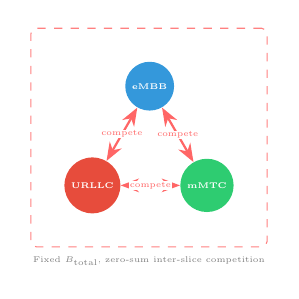
\begin{tikzpicture}[scale=0.6, transform shape,
    agent/.style={circle, minimum size=0.9cm, font=\tiny\bfseries, text=white, align=center},
]
    \node[agent, fill=embbcolor] (a1) at (90:1.4) {eMBB};
    \node[agent, fill=urllccolor] (a2) at (210:1.4) {URLLC};
    \node[agent, fill=mmtccolor] (a3) at (330:1.4) {mMTC};
    \draw[{Stealth}-{Stealth}, thick, red!60] (a1) -- node[fill=white, font=\tiny, inner sep=0.5pt] {compete} (a2);
    \draw[{Stealth}-{Stealth}, thick, red!60] (a2) -- node[fill=white, font=\tiny, inner sep=0.5pt] {compete} (a3);
    \draw[{Stealth}-{Stealth}, thick, red!60] (a3) -- node[fill=white, font=\tiny, inner sep=0.5pt] {compete} (a1);
    \node[draw=red!50, dashed, rounded corners=2pt, fit=(a1)(a2)(a3), inner sep=12pt] (box) {};
    \node[font=\tiny, text=gray, below=2pt of box] {Fixed $B_{\mathrm{total}}$, zero-sum inter-slice competition};
\end{tikzpicture}

{\tiny\textbf{Attemps}: (1) Reproducible Gymnasium-based 5G slicing simulation; (2) LangGraph-orchestrated two-tier MAS framework with proposal-evaluation-negotiation protocol.}
\end{columns}
\end{frame}


% ==================== P4 ====================
\section{Methodology}
\begin{frame}{Methodology: Architecture $\cdot$ Two-Tier Scheduling $\cdot$ Negotiation}
\begin{columns}[T]
\column{0.52\textwidth}

{\tiny\textbf{System Architecture} --- Agent Layer / Collaboration Layer (LangGraph) / Environment Layer (Gymnasium):}
\vspace{1pt}

\centering
\includegraphics[width=0.78\linewidth]{{"System Architecture.drawio"}.png}

\vspace{2pt}
{\tiny\textbf{Negotiation Flow} (LangGraph StateGraph, max 3 rounds):}
\vspace{1pt}

\centering
\includegraphics[width=0.78\linewidth]{{"Multi-Agent Negotiation Flow.drawio"}.png}

\vspace{2pt}
{\tiny \textbf{Strategies}: \textbf{M5-PA} Priority Arbitration (URLLC$>$eMBB$>$mMTC) \quad \textbf{M5-PC} Proportional Compromise (proportional reduction, above minimum)}

\column{0.48\textwidth}

{\tiny\textbf{Two-Tier Scheduling} --- Bridging LLM inference latency (seconds) vs network real-time requirements (milliseconds):}

\centering
\includegraphics[width=0.7\linewidth]{{"Two-Tier Scheduling"}.png}

\raggedright
\begin{table}
\centering\setlength{\tabcolsep}{1.5pt}\renewcommand{\arraystretch}{1.0}
\resizebox{\linewidth}{!}{\tiny
\begin{tabular}{clll}
\toprule
\textbf{ID} & \textbf{Method} & \textbf{Category} & \textbf{Description} \\
\midrule
M1 & Fixed-Ratio & Rule-based & Fixed 5:3:2 allocation \\
M2 & Threshold & Rule-based & SLA-triggered dynamic adjustment \\
M4 & Single-Agent LLM & Single LLM & GPT-4 + CoT (Chain-of-Thought) \\
M5-PA & Multi-Agent PA & Multi LLM & Priority arbitration negotiation \\
M5-PC & Multi-Agent PC & Multi LLM & Proportional compromise negotiation \\
\bottomrule
\end{tabular}}
\end{table}

\end{columns}
\end{frame}


% ==================== P5 ====================
\section{Experimental Results}
\begin{frame}{Experiment 1: Core Performance Comparison (RQ1)}
\vspace{-2pt}
\begin{columns}[T]
\column{0.55\textwidth}
{\tiny\textbf{Steady-State Scenario} (100 users, 100 decision cycles $\times$ 2 seeds):}
\vspace{1pt}

\begin{table}
\centering\setlength{\tabcolsep}{2pt}\renewcommand{\arraystretch}{1.0}
\resizebox{\linewidth}{!}{\tiny
\begin{tabular}{lccccccc}
\toprule
\textbf{Method} & \textbf{SLA\textsubscript{eMBB}} & \textbf{SLA\textsubscript{URLLC}} & \textbf{SLA\textsubscript{mMTC}} & $\bar{S}$ & \textbf{Fairness} & \textbf{Lat. (ms)} & \textbf{Tokens} \\
\midrule
M1-Fixed & 0.35{\tiny$\pm$0.05} & 0.52{\tiny$\pm$0.03} & 0.58{\tiny$\pm$0.07} & 0.48 & 0.893 & 0 & 0 \\
M2-Threshold & 0.31{\tiny$\pm$0.04} & 0.44{\tiny$\pm$0.02} & 0.51{\tiny$\pm$0.04} & 0.42 & 0.912 & 0 & 0 \\
M4-SingleLLM & 0.33{\tiny$\pm$0.01} & \textbf{0.90}{\tiny$\pm$0.01} & 0.22{\tiny$\pm$0.05} & 0.48 & 0.720 & 6326 & 26k \\
M5-PA & 0.21{\tiny$\pm$0.03} & 0.85{\tiny$\pm$0.06} & 0.15{\tiny$\pm$0.04} & 0.40 & 0.616 & 8065 & 125k \\
\rowcolor{blue!6}
M5-PC & 0.38{\tiny$\pm$0.03} & 0.76{\tiny$\pm$0.02} & \textbf{0.73}{\tiny$\pm$0.10} & \textbf{0.62} & \textbf{0.952} & 8033 & 125k \\
\bottomrule
\end{tabular}}
\end{table}

\vspace{2pt}
{\tiny\textbf{Burst Scenario} (eMBB users doubled at cycle 50):}
\vspace{1pt}

\begin{table}
\centering\setlength{\tabcolsep}{2pt}\renewcommand{\arraystretch}{1.0}
\resizebox{\linewidth}{!}{\tiny
\begin{tabular}{lccccccc}
\toprule
\textbf{Method} & \textbf{SLA\textsubscript{eMBB}} & \textbf{SLA\textsubscript{URLLC}} & \textbf{SLA\textsubscript{mMTC}} & $\bar{S}$ & \textbf{Fairness} & \textbf{Lat. (ms)} & \textbf{Tokens} \\
\midrule
M1-Fixed & 0.21{\tiny$\pm$0.06} & 0.63{\tiny$\pm$0.02} & 0.54{\tiny$\pm$0.08} & 0.46 & 0.831 & 0 & 0 \\
M2-Threshold & 0.19{\tiny$\pm$0.03} & 0.38{\tiny$\pm$0.01} & 0.45{\tiny$\pm$0.05} & 0.34 & 0.876 & 0 & 0 \\
M4-SingleLLM & 0.24{\tiny$\pm$0.02} & \textbf{0.95}{\tiny$\pm$0.00} & 0.24{\tiny$\pm$0.14} & 0.48 & 0.660 & 6063 & 26k \\
M5-PA & 0.12{\tiny$\pm$0.11} & 0.89{\tiny$\pm$0.08} & 0.15{\tiny$\pm$0.03} & 0.38 & 0.541 & 7957 & 125k \\
\rowcolor{blue!6}
M5-PC & 0.28{\tiny$\pm$0.02} & 0.80{\tiny$\pm$0.06} & \textbf{0.68}{\tiny$\pm$0.06} & \textbf{0.59} & \textbf{0.924} & 7887 & 125k \\
\bottomrule
\end{tabular}}
\end{table}

\column{0.45\textwidth}

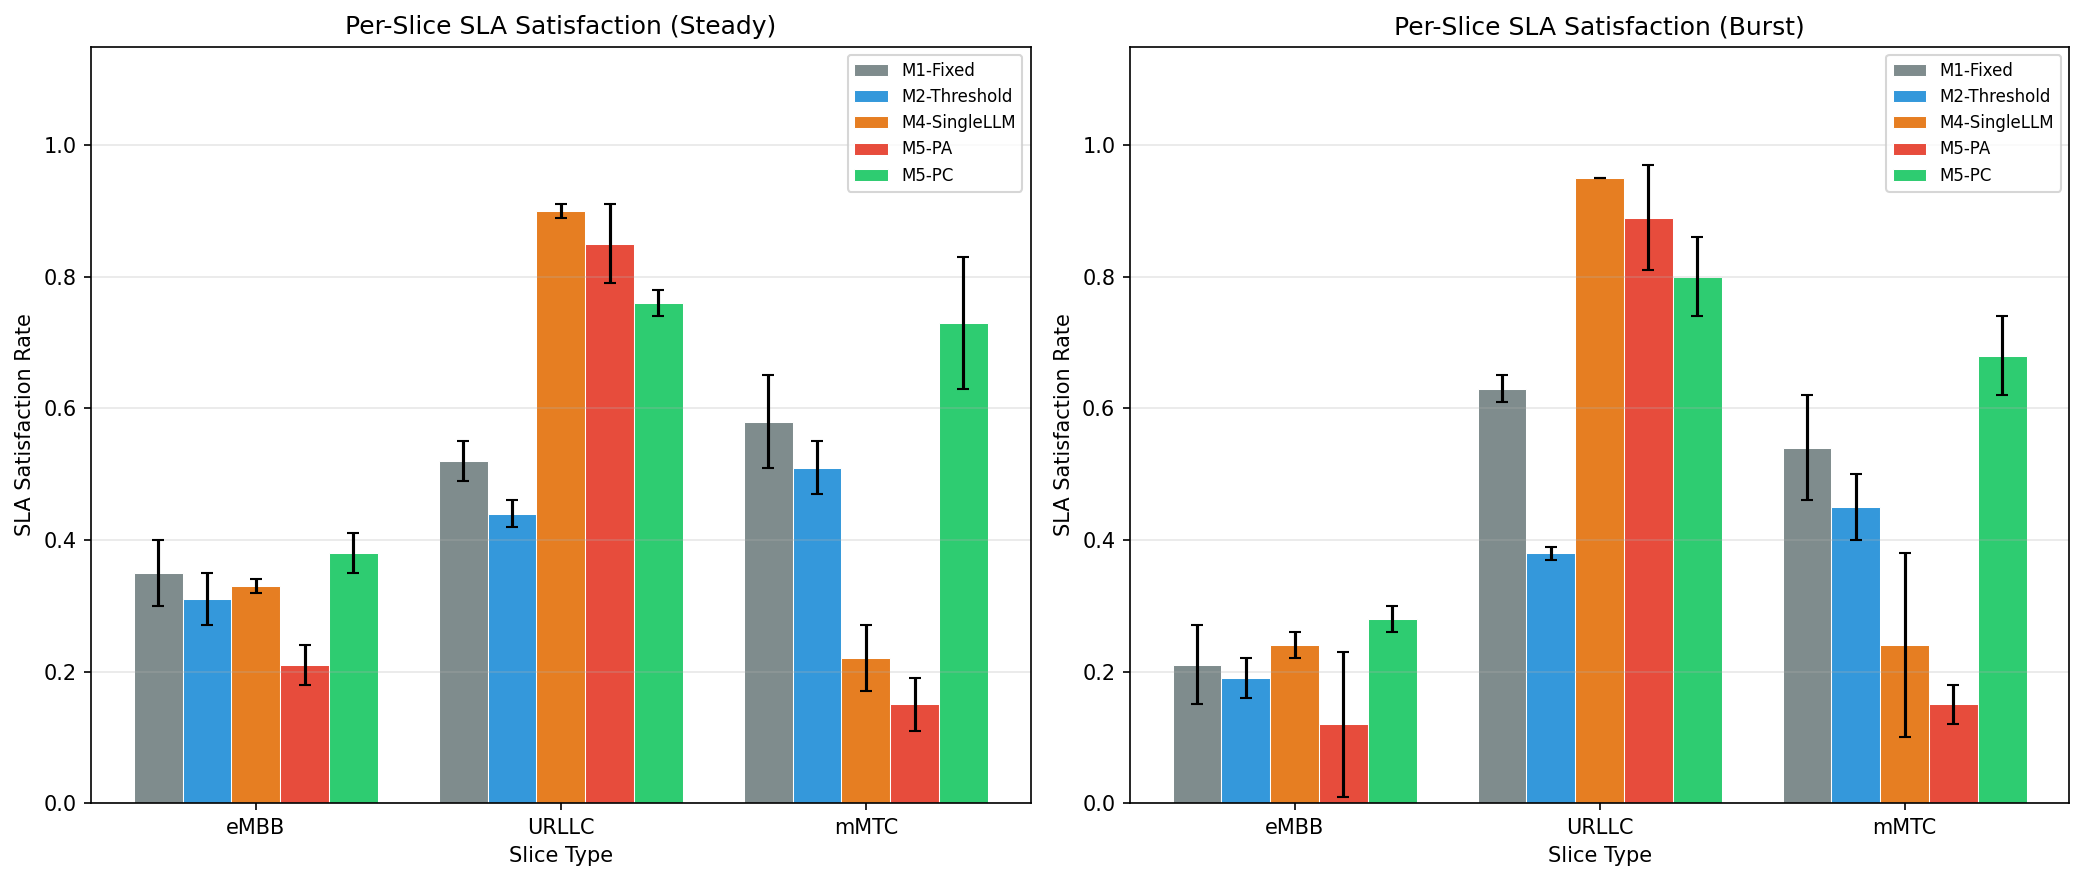
\includegraphics[width=0.95\linewidth]{slides_exp1_sla_comparison.png}

\vspace{1pt}

\begin{tcolorbox}[colback=blue!3, colframe=solcolor, boxrule=0pt, leftrule=2pt, arc=0pt, left=2pt, right=2pt, top=1pt, bottom=1pt]
\tiny
\textbf{Key Findings (RQ1):}
\begin{itemize}
\item \textbf{M5-PC} outperforms all baselines in overall SLA ($\bar{S}$=0.62) with Fairness=0.952, far above M4 (0.720) and M5-PA (0.616)
\item M5-PA over-prioritises URLLC at the expense of eMBB/mMTC
\item M4 tends toward extreme allocation: very high URLLC (0.90) but very low mMTC (0.22)
\item Rule methods have zero latency but cannot reason about SLA semantics
\item \textbf{Proportional compromise is the best strategy for balancing SLA and fairness}
\end{itemize}
\end{tcolorbox}

\end{columns}
\end{frame}


% ==================== P6 ====================
\begin{frame}{Experiment 2: Negotiation Mechanism Validation (RQ2)}
\vspace{-2pt}
\begin{columns}[T]
\column{0.42\textwidth}

\begin{table}
\centering\setlength{\tabcolsep}{2pt}\renewcommand{\arraystretch}{1.0}
\resizebox{\linewidth}{!}{\tiny
\begin{tabular}{llccccc}
\toprule
\textbf{Method} & \textbf{Scenario} & \textbf{SLA\textsubscript{eMBB}} & \textbf{SLA\textsubscript{URLLC}} & \textbf{SLA\textsubscript{mMTC}} & $\bar{S}$ & \textbf{Fairness} \\
\midrule
M5-PA & steady & 0.21 & 0.85 & 0.15 & 0.40 & 0.616 \\
M5-PA & burst & 0.12 & 0.89 & 0.15 & 0.38 & 0.541 \\
\midrule
\rowcolor{blue!6}
M5-PC & steady & 0.38 & 0.76 & 0.73 & \textbf{0.62} & \textbf{0.952} \\
\rowcolor{blue!6}
M5-PC & burst & 0.28 & 0.80 & 0.68 & \textbf{0.59} & \textbf{0.924} \\
\midrule
M5-NoNeg & steady & 0.56 & 0.49 & 0.14 & 0.39 & 0.810 \\
M5-NoNeg & burst & 0.32 & 0.71 & 0.36 & 0.46 & 0.839 \\
\bottomrule
\end{tabular}}
\end{table}

\vspace{1pt}
\centering

\includegraphics[width=0.8\linewidth]{exp2_fairness_comparison.png}

\column{0.58\textwidth}


\includegraphics[width=0.95\linewidth]{exp2_sla_per_slice.png}

\vspace{1pt}

\begin{tcolorbox}[colback=blue!3, colframe=solcolor, boxrule=0pt, leftrule=2pt, arc=0pt, left=2pt, right=2pt, top=1pt, bottom=1pt]
\tiny
\textbf{Key Findings (RQ2) --- Structural Advantage of Negotiation:}
\begin{itemize}
\item \textbf{M5-PC vs M5-NoNeg (steady)}: $\bar{S}$ +59\% (0.39$\to$0.62), Fairness +18\% (0.81$\to$0.95)
\item \textbf{M5-PC vs M5-PA}: Proportional compromise outperforms priority arbitration across all metrics, especially mMTC SLA (0.73 vs 0.15)
\item M5-NoNeg uses LLM but lacks iterative negotiation, resulting in imbalanced allocation (eMBB=0.56, mMTC=0.14)
\item M5-PA hard priority causes URLLC to monopolise resources (0.85+); low-priority slices are systematically under-served
\item \textbf{Conclusion}: The negotiation protocol itself (not merely more LLM calls) drives significant SLA and fairness improvements
\end{itemize}
\end{tcolorbox}

\end{columns}
\end{frame}


% ==================== P7 ====================
\section{Problems, Solutions \& Future Work}
\begin{frame}{Problems \& Solutions $\cdot$ Future Work}
\begin{columns}[T]
\column{0.52\textwidth}

\begin{alertblock}{\scriptsize Identified Problems}
\scriptsize
\begin{itemize}
\item \textbf{MAS latency incompatible with real-time control.} Multi-agent negotiation takes $\sim$8\,s per step, far exceeding the millisecond-level response time required by network control loops.

\vspace{3pt}
\item \textbf{Statistical significance.} Current experiments use only 2 random seeds with 100 decision cycles per episode, which limits the robustness of conclusions.
\end{itemize}
\end{alertblock}

\vspace{3pt}

\begin{exampleblock}{\scriptsize Proposed Solutions}
\scriptsize
\begin{itemize}
\item \textbf{Strategic MAS + tactical rule executor} \textit{(in progress)}: Reposition MAS as a \textbf{strategic layer} that predicts traffic trends and generates allocation \textit{policies}, rather than making per-TTI decisions. The lower-tier rule executor operates at 10\,ms granularity guided by MAS-provided policies, decoupling LLM inference from the real-time control loop.

\vspace{3pt}
\item \textbf{Expanded experimental scale}: Increase to 5 random seeds $\times$ 500 decision cycles per episode to strengthen statistical validity.
\end{itemize}
\end{exampleblock}

\column{0.48\textwidth}

\begin{block}{\scriptsize Future Work}
\scriptsize
\begin{itemize}
\item \textbf{Strategic MAS + tactical rule executor}: Validate the two-tier paradigm where MAS provides medium-term allocation policies and the rule layer handles real-time execution
\item \textbf{DRL baseline (M3-PPO)}: Train PPO (Proximal Policy Optimisation) with Stable-Baselines3 as an additional baseline
\item \textbf{RAG (Retrieval-Augmented Generation) integration}: Inject 3GPP specifications and telecom domain knowledge into agent prompts
\item \textbf{Agent memory}: Leverage historical allocation patterns to improve decision quality over time
\end{itemize}
\end{block}

\vspace{4pt}
{\tiny\textbf{Setup}: 100\,MHz (NR n78), 100 users, GPT-4o-mini (temp=0), negotiation $\leq$ 3 rounds, Gymnasium + LangGraph.}

\end{columns}
\end{frame}


% ==================== References ====================
\begin{frame}{References}
\tiny
\printbibliography[heading=none]
\end{frame}

% ==================== P8 ====================
\begin{frame}[plain]
\centering
\vspace{1cm}
{\Huge \textbf{Thank You!}}
\vspace{1em}
\end{frame}


% ============================================================
% Appendix
% ============================================================
\appendix
\section*{Appendix}

\begin{frame}{Appendix A: Simulation Environment Validation}
\begin{columns}[c]
\column{0.33\textwidth}
\centering
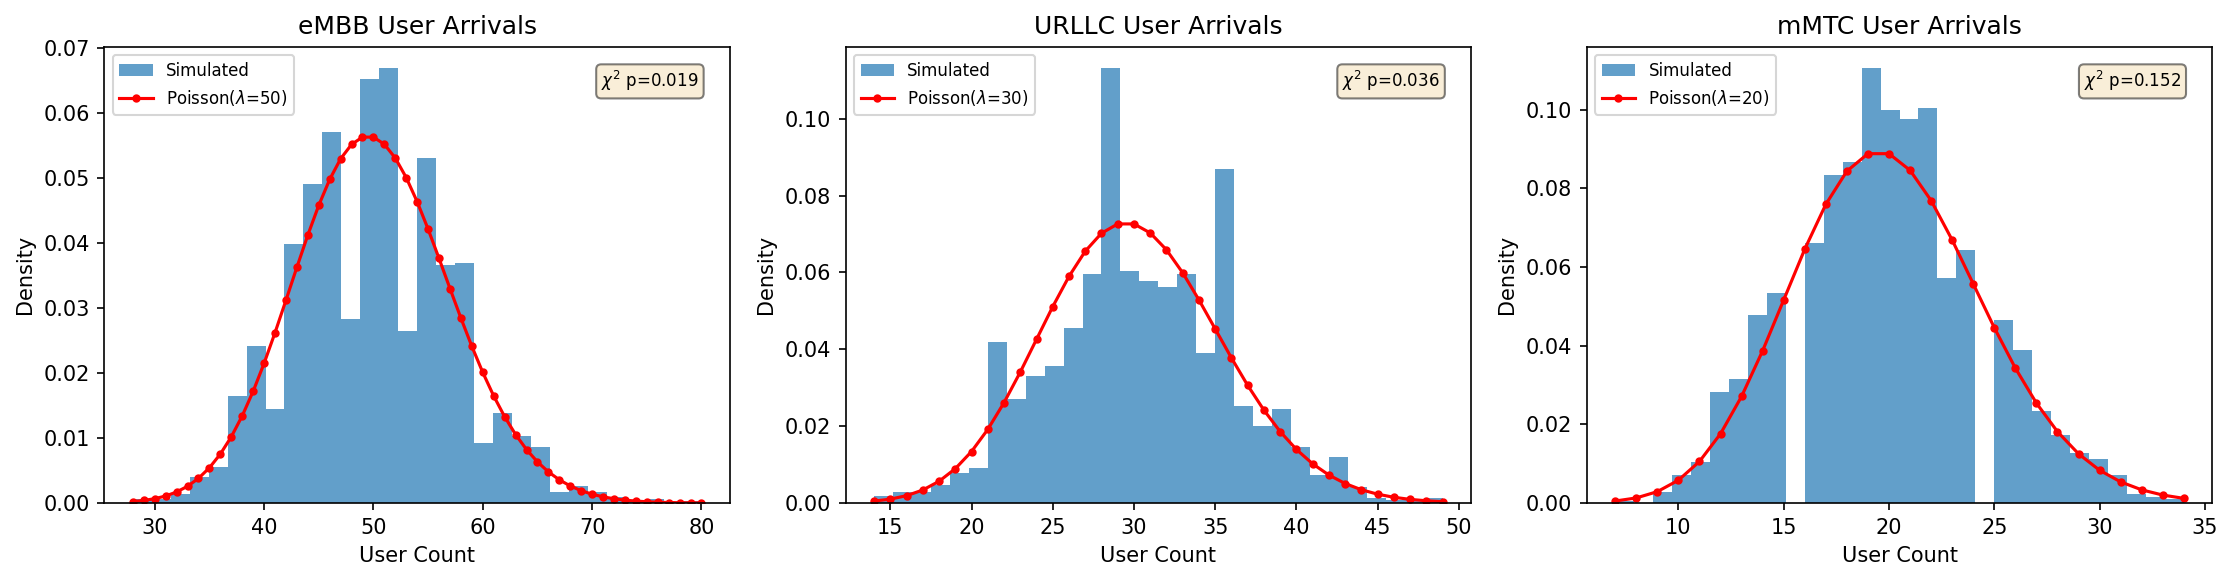
\includegraphics[width=0.9\linewidth]{validate_poisson_arrivals.png}\\
{\tiny Poisson arrival validation ($\chi^2$ test)}

\column{0.33\textwidth}
\centering
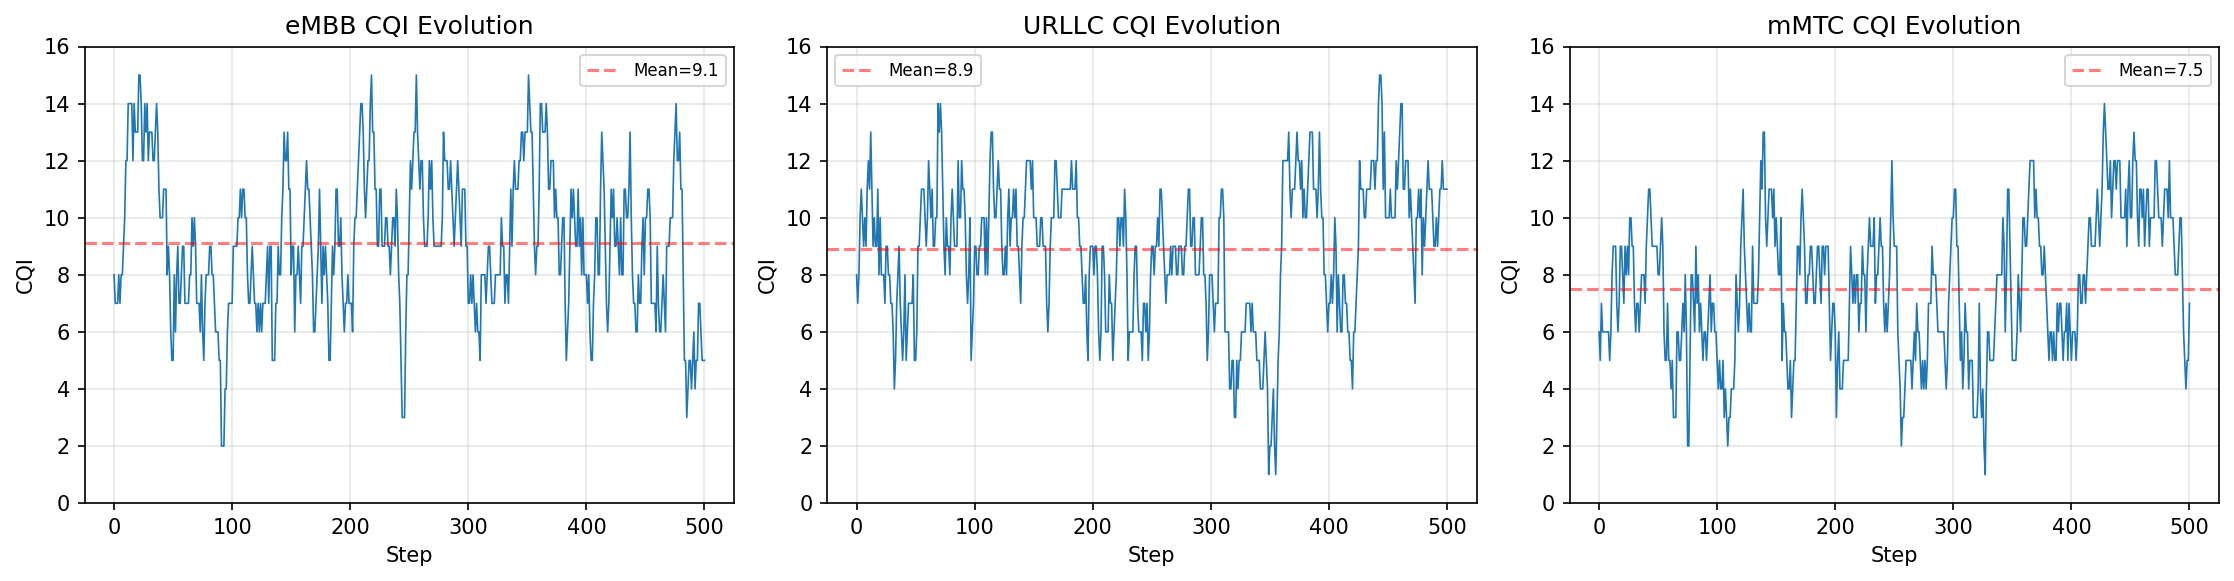
\includegraphics[width=0.9\linewidth]{validate_cqi_markov.png}\\
{\tiny CQI AR(1) mean-reverting evolution}

\column{0.33\textwidth}
\centering
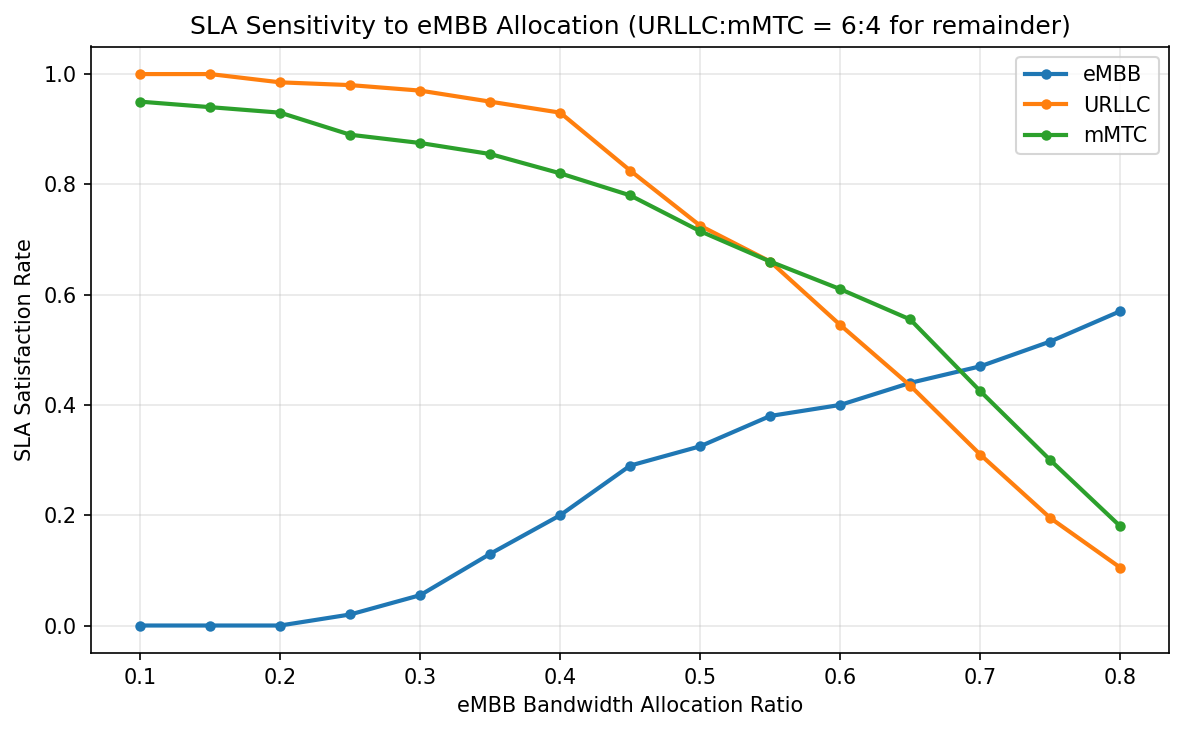
\includegraphics[width=0.9\linewidth]{validate_allocation_sensitivity.png}\\
{\tiny SLA sensitivity to allocation}
\end{columns}

\vspace{2pt}

\begin{columns}[c]
\column{0.5\textwidth}
\centering
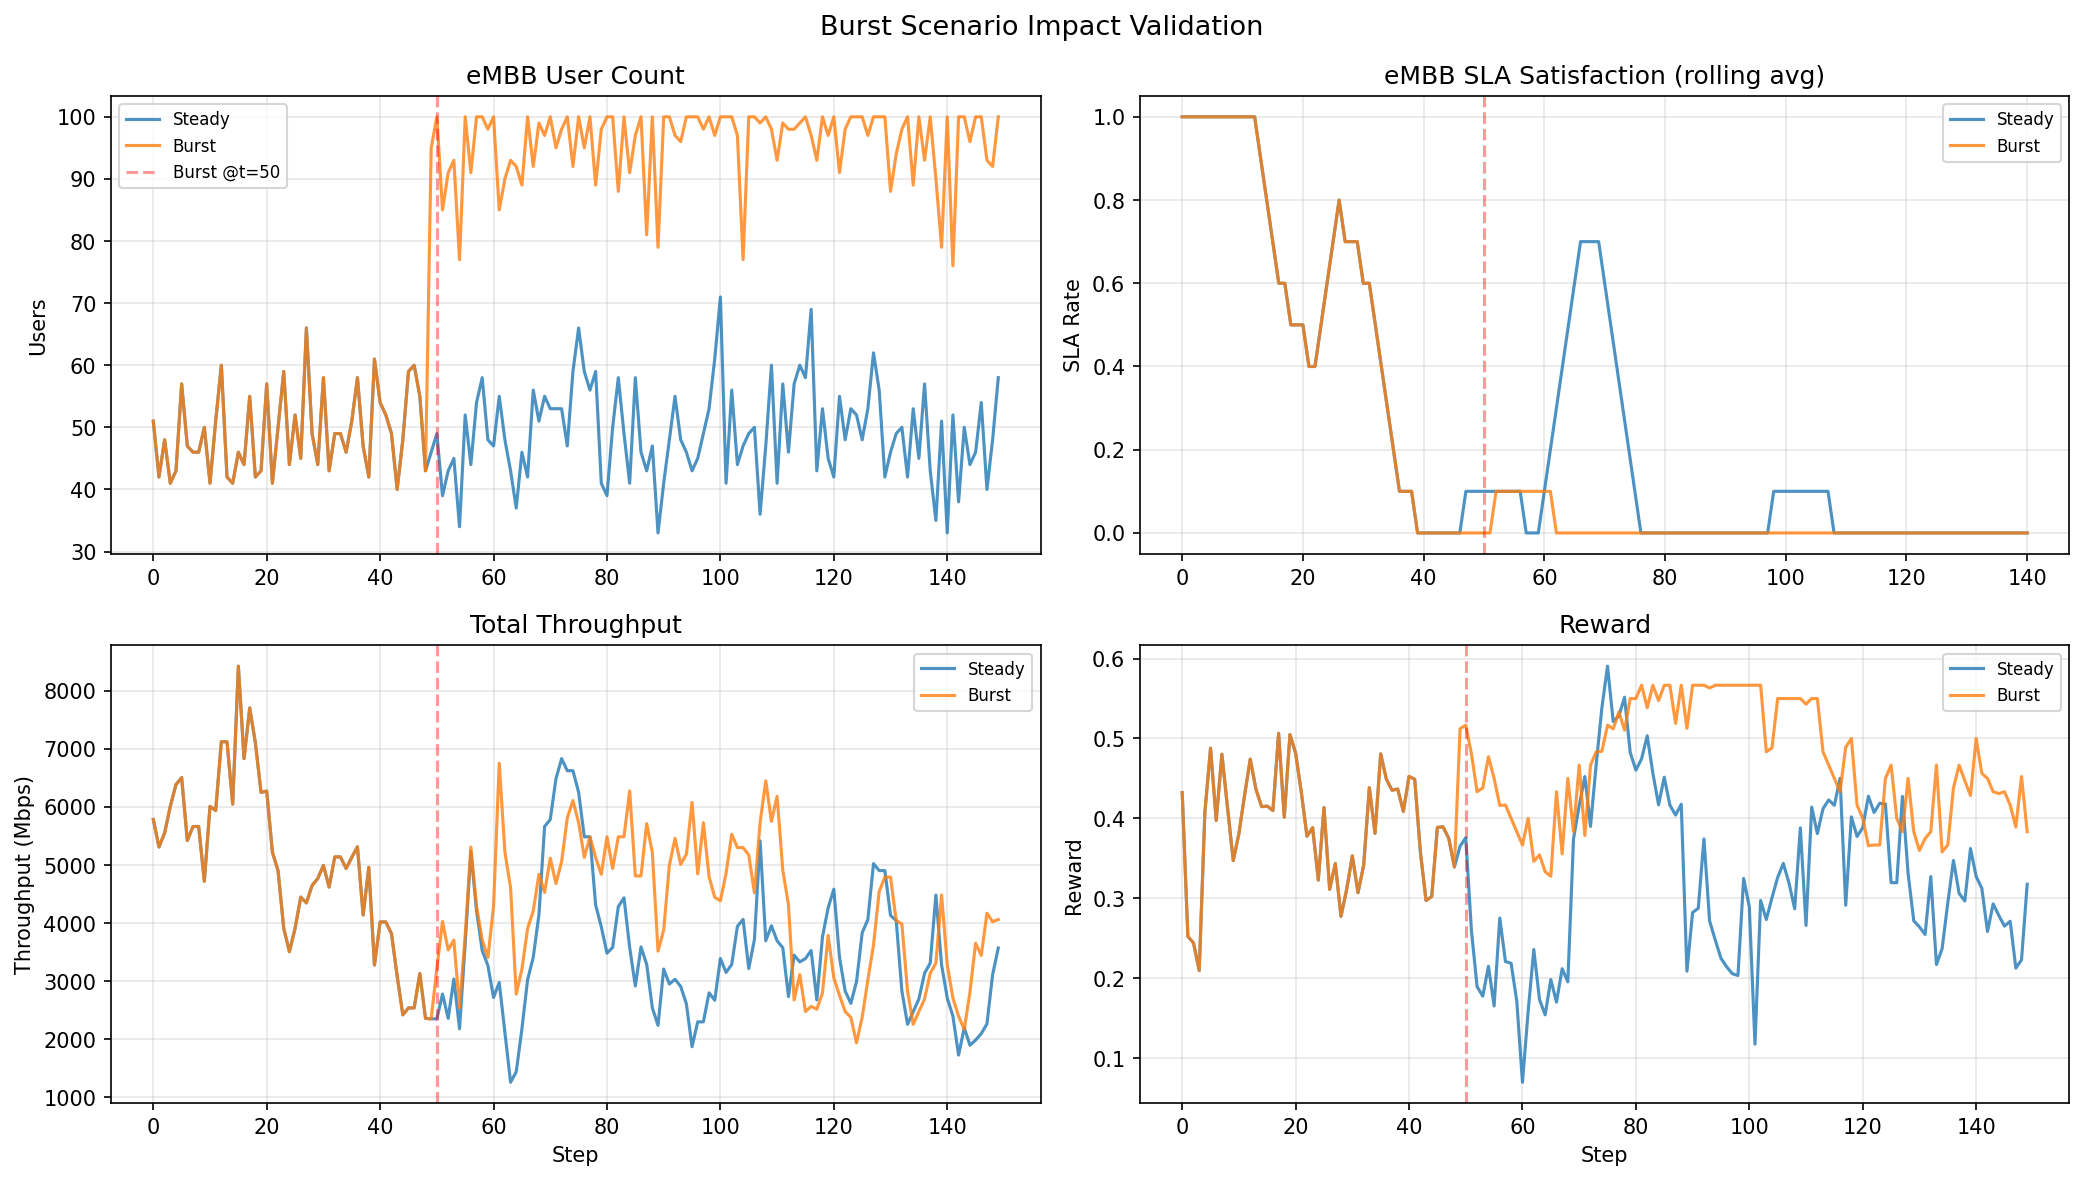
\includegraphics[width=0.72\linewidth]{validate_burst_impact.png}\\
{\tiny Burst event impact validation}

\column{0.5\textwidth}
\centering
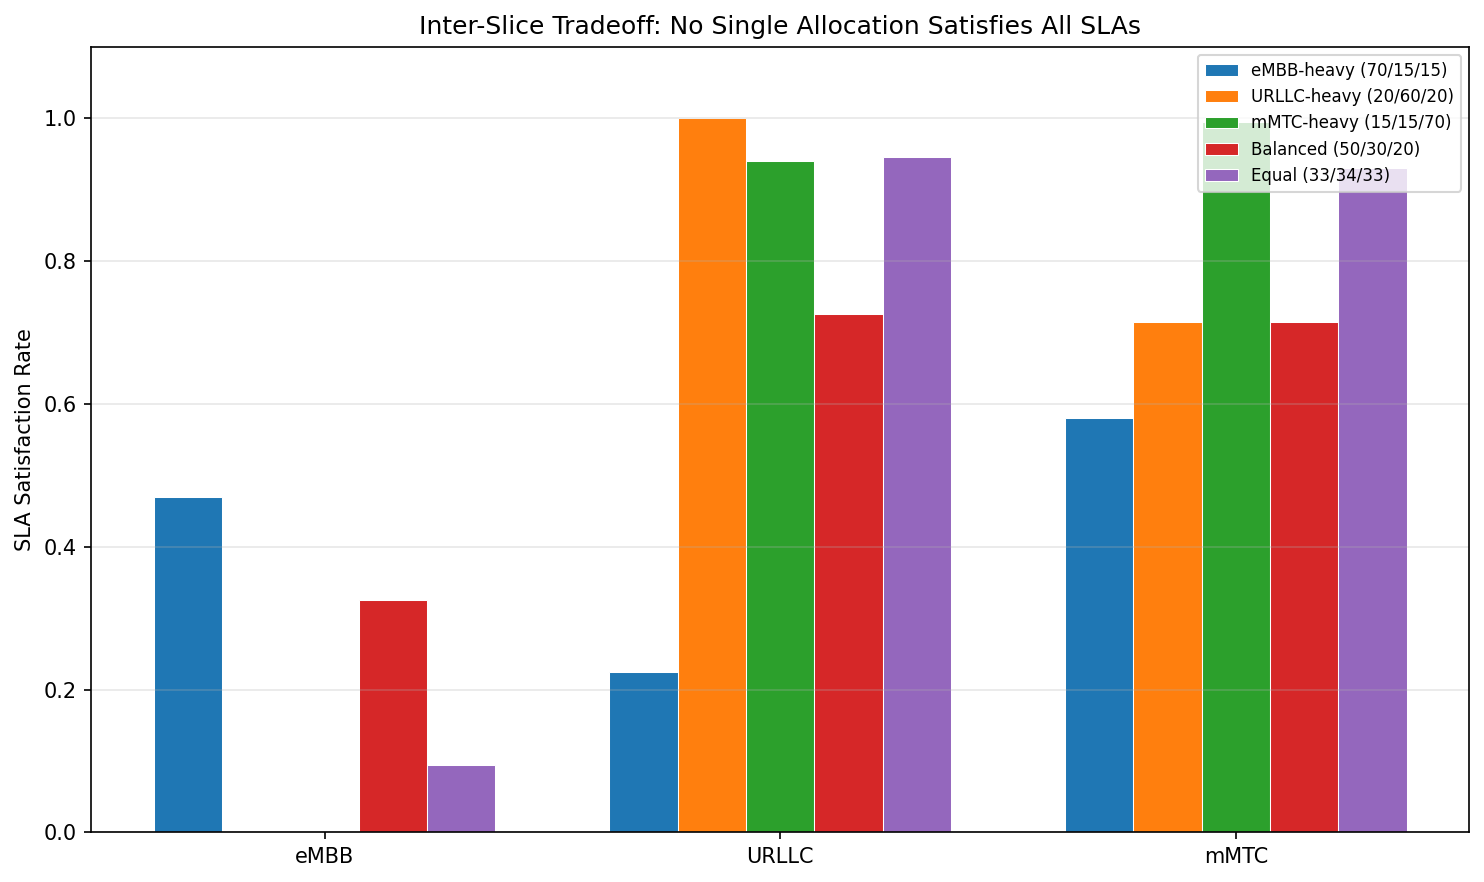
\includegraphics[width=0.72\linewidth]{validate_tradeoff.png}\\
{\tiny Inter-slice resource competition tradeoff}
\end{columns}
\end{frame}

\begin{frame}{Appendix B: Experiment 1 --- Comprehensive Performance Overview}
\centering
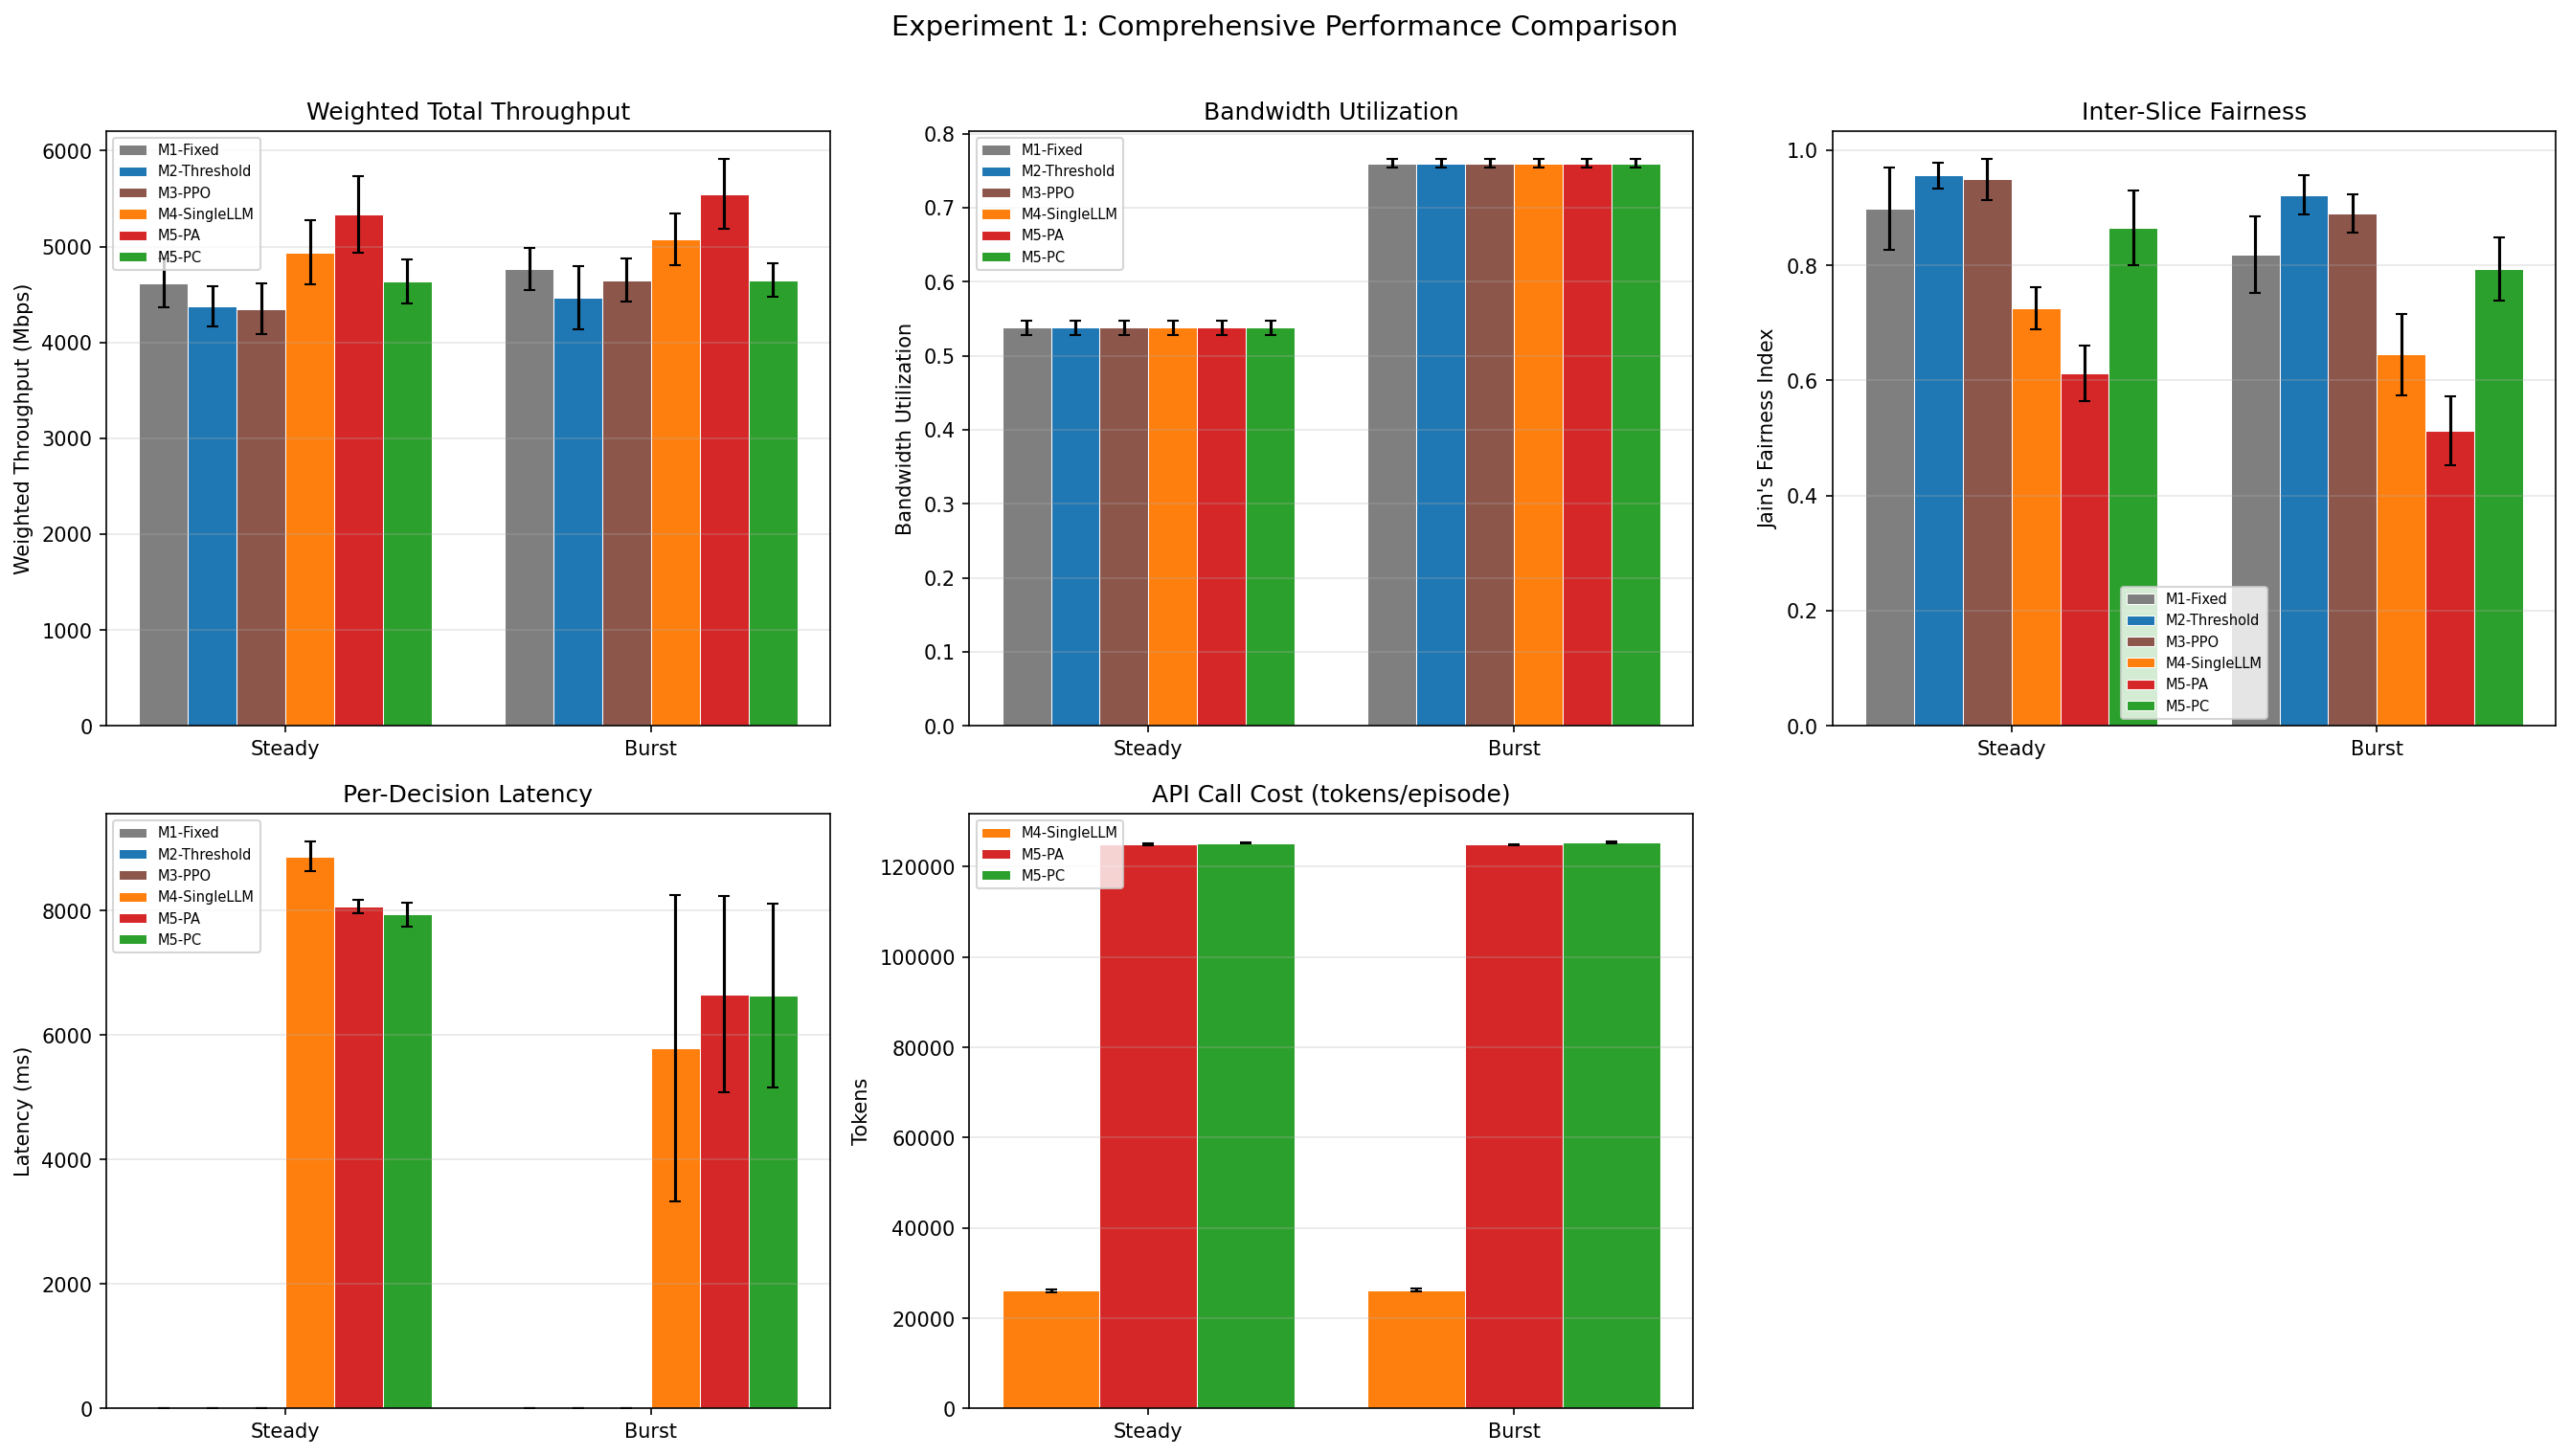
\includegraphics[width=0.68\linewidth]{exp1_performance_overview.png}\\
{\scriptsize Throughput, bandwidth utilisation, fairness, decision latency, and API cost across all five methods}
\end{frame}

\begin{frame}{Appendix C: Experiment 1 --- Burst Scenario SLA Trend}
\centering

\includegraphics[width=0.6\linewidth]{exp1_burst_trend.png}\\
{\scriptsize SLA satisfaction rate over decision cycles under burst scenario (eMBB users doubled at cycle 50)}
\end{frame}

\begin{frame}{Appendix D: Experiment 2 --- Comprehensive Performance Overview}
\centering
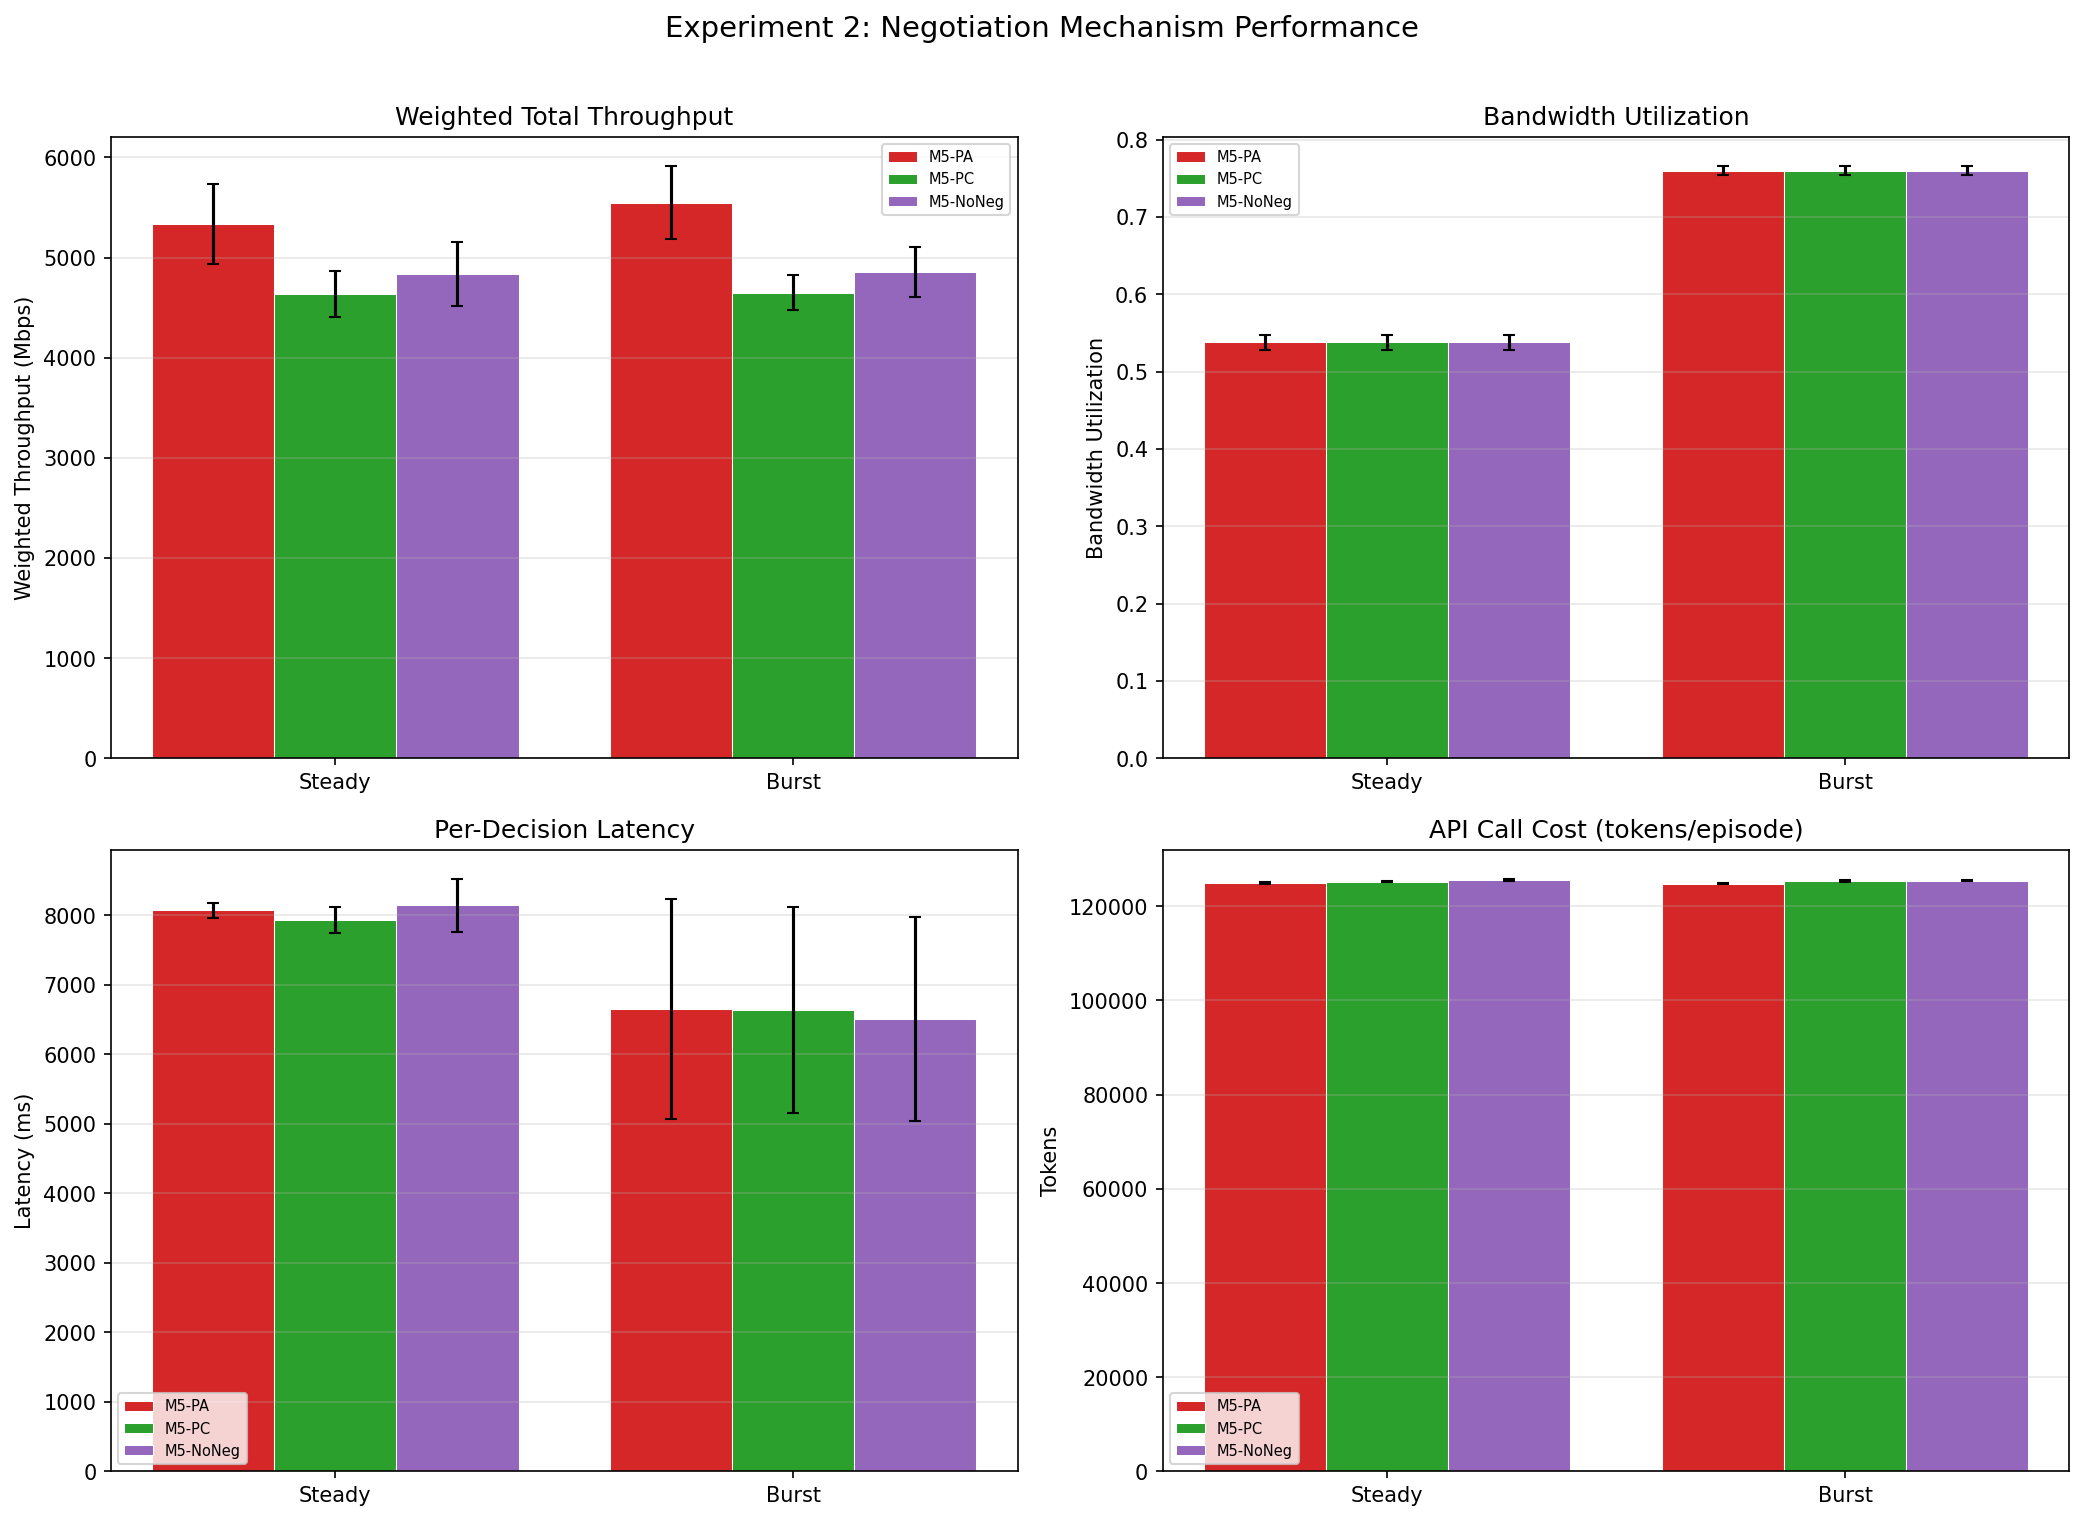
\includegraphics[width=0.5\linewidth]{exp2_performance_overview.png}\\
{\scriptsize M5-PA / M5-PC / M5-NoNeg throughput, utilisation, latency, and API cost comparison}
\end{frame}

\end{document}
